44. \begin{figure}[ht!]
\center{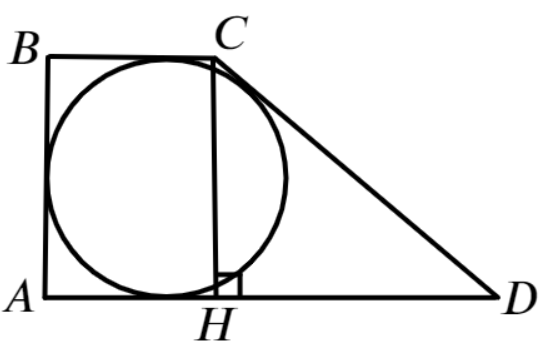
\includegraphics[scale=0.35]{g8-43.png}}
\end{figure}\\
Так как трапеция является описанным четырёхугольником, суммы её противоположных сторон равны. Проведём высоту $CH,$ тогда $HD=AD-AH=AD-BC=3-2=1,$ $CH=AB.$ Пусть $AB=x,$ тогда $AB+CD=BC+AD,\ CD=BC+AD-AB=3+2-x=5-x.$ По теореме Пифагора для треугольника $CHD$ имеем $x^2+1^2=(5-x)^2,\ x^2+1=25-10x+x^2,\ x=2,4$см. Тогда $R=\cfrac{1}{2}\cdot CH=\cfrac{1}{2}\cdot 2,4=1,2$см.\\
